\documentclass[10pt,a4paper]{article}
\usepackage[T1]{fontenc}
\usepackage[brazil]{babel}
\usepackage[utf8]{inputenc}


\usepackage{ae,aecompl}
\usepackage{pslatex}
\usepackage{epsfig}
\usepackage{geometry}
\usepackage{url}
\usepackage{textcomp}
\usepackage{ae}
\usepackage{subfig}
\usepackage{indentfirst}
\usepackage{textcomp}
\usepackage{color}
\usepackage{setspace}
\usepackage{verbatim}
\usepackage{amsmath}
%  ABACO -- Conjunto de macros para desenhar o 'abaco

%  Desenho original de Hans Liesenberg

%  Macros de Tomasz Kowaltowski

%  DCC -- IMECC -- UNICAMP

%  Mar,co de 1988  --  Vers~ao 1.0

% Ajustado para LaTeX da SUN -- Mar,co de 1991

% ---------------------------------------------------------

%  Chamada:   \ABACO{d1}{d2}{d3}{d4}{esc}
%             com:  di's -- os quatro d'igitos;
%	           esc  -- fator de escala

% ---------------------------------------------------------

%  DEFINI,C~OES AUXILIARES

% ---------------------------------------------------------


%  Forma o d'igito pequeno (0 ou 1)

\newcommand{\ABACODP}[1]{%
%
\thicklines
%    
\begin{picture}(8,0)
    \ifcase#1{   %  caso 0
       \put(0,0)    {\line(1,0){4}}
       \multiput(5,0)(2,0){2}{\oval(2,4)}}
    \or{         %  caso 1
       \put(2,0)    {\line(1,0){4}}
       \multiput(1,0)(6,0){2}{\oval(2,4)}}
    \fi
\end{picture}
    } % \ABACODP

% Forma o d'igito grande (0 a 4)

\newcommand{\ABACODG}[1]{%
%
\thicklines
%    
\begin{picture}(14,0)
    \ifcase#1{   % caso 0
       \multiput(1,0)(2,0){5}{\oval(2,4)}}
       \put(10,0)   {\line(1,0){4}}
    \or{         % caso 1
       \multiput(1,0)(2,0){4}{\oval(2,4)}}
       \put(8,0)   {\line(1,0){4}}
       \put(13,0)   {\oval(2,4)}
    \or{         % caso 2
       \multiput(1,0)(2,0){3}{\oval(2,4)}
       \put(6,0)   {\line(1,0){4}}
       \multiput(11,0)(2,0){2}{\oval(2,4)}}
    \or{         % caso 3
       \multiput(1,0)(2,0){2}{\oval(2,4)}
       \put(4,0)   {\line(1,0){4}}
       \multiput(9,0)(2,0){3}{\oval(2,4)}}
    \or{         % caso 4
       \put(1,0)  {\oval(2,4)}}
       \put(2,0)   {\line(1,0){4}}
       \multiput(7,0)(2,0){4}{\oval(2,4)}
    \fi
\end{picture}
    } % \ABACODG
       
% Forma um d'igito (0 a 9)

\newcommand{\ABACOD}[1]{%
%
    \ifnum#1>9
       \errmessage{#1: Argumento invalido para ABACO}
    \fi
    \ifnum#1<0
       \errmessage{#1: Argumento invalido para ABACO}
    \fi
%
\begin{picture}(24,0)
%    
    \ifnum#1<5
       \put(16,0) {\ABACODP{0}}
    \else   
       \put(16,0) {\ABACODP{1}}
    \fi
%    
    \ifnum#1<5
       \put(0,0)  {\ABACODG{#1}}
    \else
       \ifcase#1\or \or \or \or
          \or  \put(0,0)  {\ABACODG{0}}
          \or  \put(0,0)  {\ABACODG{1}}
          \or  \put(0,0)  {\ABACODG{2}}
          \or  \put(0,0)  {\ABACODG{3}}
          \or  \put(0,0)  {\ABACODG{4}}
       \fi
    \fi   
\end{picture}
    } % \ABACOD
    
% -------------------------------------------------

%  DEFINI,C~AO PRINCIPAL
    
\newcommand{\ABACO}[5]{%
    \setlength{\unitlength}{#5mm}
%
    \thinlines
%   
\begin{picture}(28,25)
%   
% moldura
%
% externa
%
        \put(0,0)            {\line(0,1){25}}
        \put(0,0)            {\line(1,0){28}}
        \put(28,0)           {\line(0,1){25}}
        \put(0,25)           {\line(1,0){28}}
% interna
        \put(2,2)            {\line(0,1){21}}
	\put(26,2)           {\line(0,1){21}}
	\put(16,2)           {\line(0,1){21}}
	\put(18,2)           {\line(0,1){21}}
	\put(2,2)            {\line(1,0){14}}
	\put(16,2)           {\line(1,-1){1}}
	\put(17,1)           {\line(1,1){1}}
	\put(18,2)           {\line(1,0){8}}
	\put(2,23)           {\line(1,0){14}}
	\put(16,23)          {\line(1,1){1}}
	\put(17,24)          {\line(1,-1){1}}
	\put(18,23)          {\line(1,0){8}}
	\put(0,0)            {\line(1,1){2}}
	\put(0,25)           {\line(1,-1){2}}
	\put(28,0)           {\line(-1,1){2}}
	\put(28,25)          {\line(-1,-1){2}}
%
%   
% d'igitos
%
%   
       \put(2,20)  {\ABACOD{#1}}
       \put(2,15)  {\ABACOD{#2}}
       \put(2,10)  {\ABACOD{#3}}
       \put(2,5)   {\ABACOD{#4}}
%      
\end{picture}
    } % \ABACO
    
 


 %\onehalfspacing
  \doublespacing
\begin{document}

% CAPA
  \thispagestyle{empty}
  
  \begin{minipage}[h]{0.10\linewidth}
    \ABACO{1}{9}{6}{9}{0.5} 
  \end{minipage}
  \begin{minipage}[h!]{0.7\linewidth}
    \vspace*{\fill}
    \centering
    {\large \textbf{UNIVERSIDADE~ESTADUAL~DE~CAMPINAS}}\\ 
    {\large INSTITUTO~DE~COMPUTAÇÃO}                   
    \vspace*{\fill} 
  \end{minipage}
    \\\vspace{0.5cm}
  
  \begin{center} 
    \rule{11.0cm}{0.4pt}\vspace*{-\baselineskip}\vspace{-2.0pt}
    \rule{11.0cm}{1.6pt} \vspace*{-\baselineskip}
      {\Large \textsc{Reconhecimento de faces em redes sociais}}\vspace{3.2pt}
    \rule{11.0cm}{0.4pt}\vspace*{-\baselineskip}\vspace{3.2pt} \rule{11.0cm}{1.6pt}\\
    {\textsl{Proposta de projeto}}
    \\\vspace{1cm}
    \begin{tabular}{ll}
      Carlos Eduardo Rosa Machado & \textbf{RA}: 059582\\
       \multicolumn{2}{c}{\small \emph ra059582@students.ic.unicamp.br}  \\
      Douglas Alves Germano        & \textbf{RA}: 060210\\
      \multicolumn{2}{c}{\small \emph ra060210@students.ic.unicamp.br } \\
      Tiago Chedraoui Silva        & \textbf{RA}: 082941\\
      \multicolumn{2}{c}{\small \emph ra082941@students.ic.unicamp.br} \\
    \end{tabular}
  \end{center}
  \vspace{0.5cm}
 \tableofcontents
\newpage 
  \section{Introdução e Motivação}

	Rede social é uma estrutura composta por indivíduos ou organizações, chamados de nós, que se conectam por um ou vários tipos de relações, tais como amizade, parentesco, interesses em comum, entre outras.
	
	O Facebook é uma rede social gratuita, fundada em 2004, e atualmente possui mais de 700 milhões de usuários ativos.

	Uma pessoa pode criar um perfil na rede social, tornando-se um
        usuário do sistema. Para a criação de um perfil, ela deve
        fornecer informações pessoais como nome, localização, endereço
        eletrônico, e outras que desejar. Entre as opções, o usuário
        pode fornecer uma foto para ser mostrada no perfil, que
        qualquer outro usuário terá acesso irrestrito e a
        possibilidade de visualizá-la. Ainda assim, esta é uma prática
        bastante utilizada pela maioria dos usuários, pois proporciona
        fácil reconhecimento pelas demais pessoas. Além disso, o
        usuário pode colocar outras fotos pessoais, para as quais
        controlará o acesso, deixando restrito, por exemplo, apenas para aqueles que fazem parte da sua rede de relacionamentos no sistema.

	Pelo próprio intuito da rede, um usuário cadastrado quer se conectar e se relacionar virtualmente com as pessoas que conhece, ou até mesmo conhecer pessoas novas, quando algum interesse mútuo ocorre.

	Desta forma, o Facebook tem algumas ferramentas à disposição dos usuários, que permitem pessoas serem encontradas por outras usando alguma informação, tal como nome, endereço eletrônico ou endereço físico.

	Por isso, a ambição do projeto está em criar uma nova
        ferramenta, um novo meio para que as pessoas se encontrem e se
        conheçam. Apesar do Facebook ter bons buscadores que encontram
        facilmente uma pessoa, precisamos sempre ter alguma informação
        da pessoa, que podemos não saber e não conseguir obter
        rapidamente. Contudo, podemos ter uma foto, e é neste caso que
        entra a nossa proposta de solução: buscar um perfil dado uma
        foto.
\newpage
  \section{O problema}

	Participar ativamente de uma rede social, tal qual o Facebook, está muito ligado em encontrar seus amigos online e fazer novos amigos, para assim trocar mensagens com os usuários, participar de eventos, estar presente em grupos, entre outras possibilidades. Por conseguinte, o problema consiste em conectar estes usuários, de modo que amigos recentes ou velhos amigos possam ser encontrados facilmente.

	É esperado que uma pessoa saiba, ou tenha anotado em algum lugar, informações básicas sobre seus amigos. Porém, nem sempre nos recordamos ou temos estes dados em mãos. Por exemplo, você acabou de conhecer uma pessoa, que por falta de tempo ou por distração, não perguntou o nome dela. Mas, como estavam numa festa e você tirou diversas fotos, acabou reconhecendo ela em uma das diversas fotos que nem se lembra de ter tirado. Assim, com as atuais ferramentas que o Facebook disponibiliza, você não seria capaz de encontrá-la facilmente, pois não sabe nada sobre a pessoa.

A proposta deste projeto é incluir uma ferramenta diferente, que não precisa de qualquer tipo de informação sobre o indivíduo, mas que seja capaz de encontrá-lo por comparação da imagem alvo, esta que você possui na sua câmera, com as imagens dos perfis dos usuários.

	Ou seja, o usuário fornece a foto com o rosto da pessoa que deseja buscar, o sistema (e eventualmente um aplicativo) varre a rede procurando as imagens mais semelhantes e retorna os perfis que contém os rostos mais parecidos, e eventualmente, o perfil correto do usuário buscado.

	De início, surgem dois problemas: encontrar uma face dado uma imagem e encontrar esta face em outras imagens. Dado que temos isto, uma ferramenta capaz de reconhecer as características de um ser humano e recortar seu rosto, e outra que faça a comparação das faces detectadas, surge um problema bônus: a imensa quantidade de usuários cadastrados no Facebook.

	São centenas de milhões de pessoas ativas especificamente no Facebook, e portanto, fazer a comparação entre todos estes usuários em tempo razoável é uma outra dificuldade a ser enfrentada.

	Deste modo, este projeto se propõe a fornecer um novo meio de encontrar usuários na rede utilizando apenas uma foto, mas que dê algum resultado, seja ele de sucesso ou fracasso, em um tempo hábil, mantendo a satisfação do cliente.

	Existem outros problemas com os quais lidaremos, mas que não temos muito o que fazer para saná-los, tais como: perfil criado sem foto ou que a foto não seja da pessoa, imagens ruins, ou então que não contenha um rosto.

\section{Solução proposta}
A abordagem tomada foi de criar um aplicativo externo ao Facebook, que utiliza das formas de conexões desenvolvidas e publicadas pela empresa, para interagir e manipular os dados necessários ao nosso projeto.

\subsection*{Definição do espaço:}

	A primeira precaução do grupo foi definir o espaço de busca do algoritmo. Dado que o Facebook registra em torno de 700 milhões de usuários ativos no sistema, fazer a comparação entre todos e retornar um resposta adequada seria improvável, pois algoritmos semelhantes, como o do Picasa, demora 6 dias para comprar 50 mil fotos, tempo totalmente fora do esperado pelo usuário.

	Portanto, partimos da premissa que a pessoa buscada talvez seja um amigo de um amigo do usuário e limitamos nesta fronteira. Se um usuário médio tem em torno de 130 amigos na rede, estaríamos nos propondo a realizar a busca por 16900 usuários (130 x 130) no caso médio. Esta abordagem nos pareceu bastante favorável, para um retorno satisfatório num tempo adequado.

\subsection*{Graph API:}

	O Facebook disponibiliza uma plataforma de desenvolvimento para qualquer pessoa que esteja interessado em iniciar um programa e utilizar das informações contidas nos perfis dos usuários. Vale ressaltar que nem todos os dados pessoais são públicos, a menos que o usuário habilite para que sejam. Entretanto, ao menos a foto do seu perfil, ponto de interesse do projeto, será visualizável a qualquer um.

	Toda informação está no que eles chamam de grafo social, onde qualquer coisa é um nó, com identificador único, e possue relações com outros nós. Por exemplo, um usuário X é um nó e está conectado com outro usuário Y, também nó, por uma relação de amizade. São nós: usuários, eventos, fotos, páginas e etc. E são conexões: amizade, participação em eventos, marcação em fotos e outros.

	Tudo isto está disposto numa arquitetura de JSON facilmente entendida. Um JSON é composto por uma propriedade e seu valor. Ou seja, para um usuário teremos, por exemplo, a propriedade nome e o seu valor, seu nome.

\subsection*{Python:}

	Com as informações obtidas do Graph API, e conhecendo sua estrutura formada por JSON, optamos por utilizar python para desenvolvimento. Se mostrou interessante num primeiro momento, pela grande facilidade de realizar conexões com o Facebook e de manipular as respostas recebidas em formato JSON.

	Porém, por ser uma linguagem interpretada, ganhamos em simplicidade e perdemos em processamento, pois uma linguagem compilada seria mais veloz.


\subsection*{PCA:}

\begin{equation}
\lambda_{k}=\frac{1}{M}\sum_{n=1}^{M}(u_k^T\Phi_n)^2
\end{equation}


\begin{equation}
u_l^Tu_k=\delta_{lk}=\left \{
  \begin{array}{l l}
    1, & \quad \text{se $l=k$} \\
    0, & \quad \text{caso contrário}\\
  \end{array}
\right.
\end{equation}



\begin{equation}
C=\frac{1}{M}\sum_{n=1}^{M}(\Phi_n\Phi_n^T)= AA^T
\end{equation}


\begin{equation}
A^TAv_i=\mu_iv_i
\end{equation}



\begin{equation}
AA^TAv_i=\mu_iAv_i
\end{equation}



\begin{equation}
u_l=\sum_{k=1}^{M}(v_{lk}\Phi_k) \quad\quad\quad l = 1,...,M
\end{equation}


\begin{equation}
\omega_k=u_k^T(\Gamma-\Psi)
\end{equation}



\begin{equation}
\epsilon_k^2=\|\Omega-\Omega_k\|^2
\end{equation}


\begin{equation}
\epsilon^2=\|\Phi-\Phi_f\|^2
\end{equation}

\subsection*{Interface:}
Inicialmente, um usuário deverá fornecer uma foto contendo a pessoa a que deseja procurar. A partir da foto fornecida é feito uma busca por faces presentes nela e para cada face encontrada é fornecida a possibilidade de escolha de qual face deve-se procurar na rede social, caso nenhuma face seja encontrada, é fornecido ao usuário a possibilidade de escolha da face através de um retângulo ajustável nas proporções 4:3 (ver figura 1).

\begin{figure}[h!]
\begin{center}
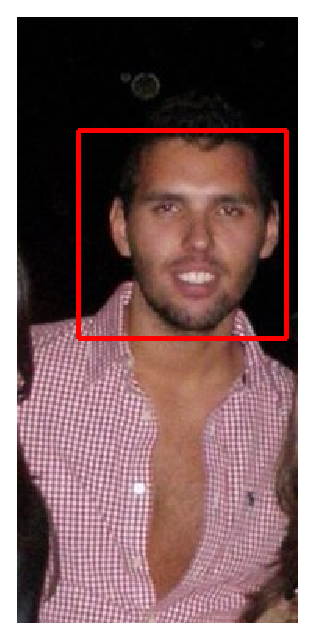
\includegraphics[scale=0.4]{samephoto}
\caption{ Seleção da face na foto fornecida}
\end{center}
\end{figure}

Após a seleção da face para busca, nosso usuário espera um tempo até que seja criada uma janela contendo as seis faces mais próximas encontradas (ver figura 2). O usuário terá a possibilidade de escolher das faces aquela que for seu o procurado, caso a face seja encontrada, ao clicar sobre a foto de perfil fornecida o usuário é redirecionado ao perfil dessa pessoa.
Pode acontecer de nehuma das faces fornecida ser a pessoa que queremos encontrar, nesse caso a janela pode ser fechada.

\begin{center}
\begin{figure}[h!]
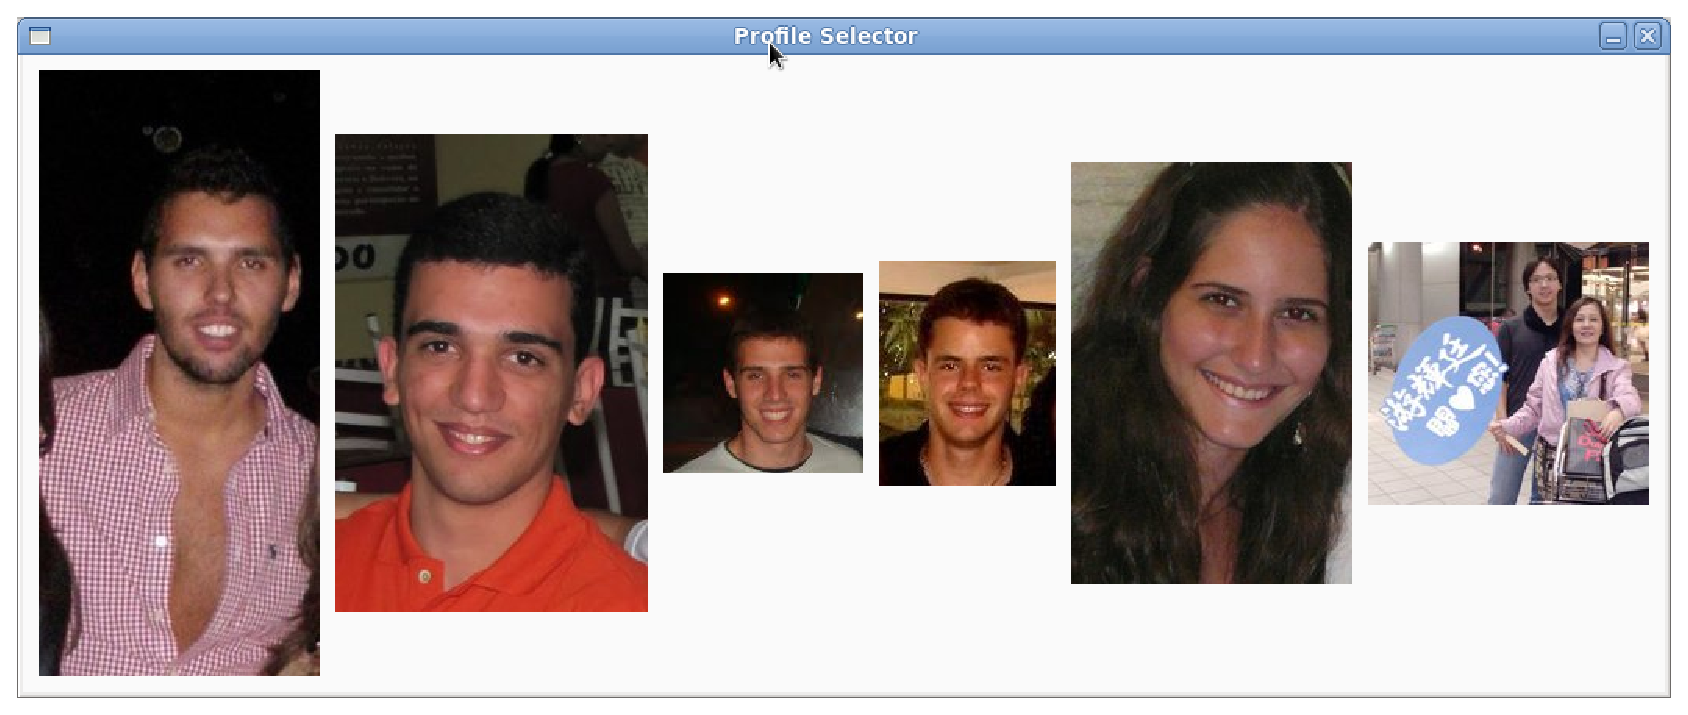
\includegraphics[scale=0.5]{6maisproximos}
\caption{Faces mais próximas}
\end{figure}
\end{center}

\section{Exprerimentos}

\section{Conclusões}

% ******************************************************
% 		REFERENCIAS BIBLIOGRÁFICAS
% ******************************************************
%\section{Referências}
\bibliographystyle{plain}
\begin{small}
  \bibliography{referencias}
\end{small}


\end{document}